% !TEX program = xelatex
\documentclass[12pt,a4paper]{article}

% 数学公式相关包
\usepackage{amsmath}
\usepackage{amsfonts}
\usepackage{amssymb}
\usepackage{mathrsfs}
\usepackage{bm}

% 其他常用包
\usepackage{graphicx}
\usepackage{geometry}
\usepackage{float}
\usepackage{caption}
\usepackage{subcaption}

% 页面设置
\geometry{left=2.5cm,right=2.5cm,top=2.5cm,bottom=2.5cm}

% 中文支持
\usepackage{ctex}

% 自定义命令
\newcommand{\diff}{\mathrm{d}} % 微分符号
\newcommand{\pdiff}{\partial} % 偏微分符号
\newcommand{\e}{\mathrm{e}} % 自然对数的底
\newcommand{\im}{\mathrm{i}} % 虚数单位
\newcommand{\bvec}[1]{\mathbf{#1}} % 粗体向量

\title{数学推导}
\author{火兴辉}
\date{\today}

\begin{document}
\maketitle

\section{无量纲量}

\subsection{密度比}
\begin{equation}
    s = \frac{\rho_p}{\rho_f}
\end{equation}
where $\rho_p$ is the particle density and $\rho_f$ is the fluid density.

\subsection{考虑浮力的有效重力加速度}
\begin{equation}
    \hat{g} = g(1-\frac{1}{s})
\end{equation}
where $g$ is the gravity acceleration.

$\sqrt{s}$ separates the settling velocity scale $\sqrt{s \hat{g} d}$ from the escape velocity scale $\sqrt{\hat{g} d}$ that grains need to exceed in order to escape the potential traps of the bed surface.

\subsection{Galileo Number}
\begin{equation}
    Ga = \frac{d \sqrt{s \hat{g} d}}{\nu_f}
\end{equation}
where $d$ is the particle diameter and $\nu_f$ is the kinematic viscosity.

$Ga$ controls the scaling of the dimensionless terminal grain settling velocity in quiescent flow $v_s^-/\sqrt{s \hat{g} d}$ (Camenen, 2007). 

\subsection{Shields Number}
\begin{equation}
    \Theta = \frac{\tau}{\rho_p \hat{g} d}
\end{equation}
where $\tau$ is the fluid shear stress on the bed surface.

The Shields Number $\Theta$ is a measure for the ratio of the shear stress on the bed surface to the effective weight of the sediment particle (P\"ahtz et al., 2020).

\subsection{空中颗粒承载量}

The transport load $M$ is the total mass of transported particles in the air per unit bed area. Non-dimensionalized by the particle density and diameter, it is defined as
\begin{equation}
    M_* = \frac{M}{\rho_p d}.
\end{equation}

\subsection{流向颗粒通量}
\begin{equation}
    Q = M \overline{v_x}
\end{equation}
where $\overline{v_x}$ is the streamwise average particle velocity. Non-dimensionalized as
\begin{equation}
    \overline{v_{x*}} = \frac{\overline{v_x}}{\sqrt{s \hat{g} d}}.
\end{equation}
while the non-dimensional streamwise particle transport rate is defined as
\begin{equation}
    Q_* = \frac{Q}{\rho_p d \sqrt{s \hat{g} d}}.
\end{equation}

\section{输沙率表达式}
P\"ahtz et al. (2020) proposed new expressions for $M_*$ and $Q_*$.
\begin{equation}
    M_* = (\Theta - \Theta_t)/\mu_b,
\end{equation}
\begin{equation}
    Q_* = M_* \overline{v_{x*}}_t (1 + c_M M_*) \label{eq:Qstar},
\end{equation}
where $\mu_b$ is the bed friction coefficient, which approximates the ratio between the average streamwise momentum loss and vertical momentum of transported particles during their contacts with the bed surface (P\"ahtz et al., 2018). The subscripts $t$ refers to the threshold value and $\Theta_t$ is the partical transport threshold (i.e., $M_* \rightarrow 0$ when $\Theta \rightarrow \Theta_t$).

Equation \ref{eq:Qstar} consists of two additive contributions to $Q_*$: the term $M_* \overline{v_{x*}}_t$ corresponds to the scaling of $Q_*$ in the hypothetical case that collisions between transported particles are ommitted, and the term $c_M M_* \overline{v_{x*}}_t$ accounts for such collisions.

P\"ahtz et al. (2020) found that Eq. \ref{eq:Qstar} with $c_M = 1.7$ is universally valid across a wide range of equilibrium non-suspended transport simulations ($s \in [2.65, 2000] and Ga \in [5, 100]$) that satisfy $s^{1/2} Ga \geq 80$ for $s \leq 10$ (typical for fluvial environments) or $s^{1/2} Ga \geq 200$ for $s \leq 10$ (typical for aeolian environments). The value of $\Theta_t$ is fitted to experimental and numerical data, while $\mu_b$ and $\overline{v_{x*}}_t$ are derived from semi-empirical relations: $\mu_b = 0.63$ (P\"ahtz and Dur\'an, 2018) and $\overline{v_{x*}}_t \approx 2 \kappa^{-1} \sqrt{\Theta_t}$ (limited to $s^{1/4} Ga \geq 40$, P\"ahtz and Dur\'an, 2018).

\section{颗粒跃移模型}
\subsection{流场廓线}
\begin{equation}
    u_x = \frac{u^*}{\kappa}ln\frac{z}{z_0} \label{eq:ux},
\end{equation}
where $u_x$ is the wind speed, $u^*$ is the friction velocity, $\kappa = 0.41$ is the von Karman constant, $z$ is the height, and $z_0=d_{90}/30$ is the roughness length.

We use non-dimensional arguments to rewrite Eq. \ref{eq:ux} as
\begin{equation}
    u_x = u^* f_u(z),
\end{equation}
with
\begin{equation}
    f_u(z) = \frac{1}{\kappa}ln\frac{z}{z_0}.
\end{equation}
\subsection{流场对颗粒的拖曳力}
Define the fluid velocity as $\vec{u}$ and the particle velocity as $\vec{v}$. Considering the particle as a rigid sphere, the drag force exerted by the fluid on the particle can be expressed as
\begin{equation}
    F_d = \frac{\pi}{8} \rho_f C_d d^2 |\vec{u} - \vec{v}| (\vec{u} - \vec{v}),
\end{equation}
where $C_d$ is the drag coefficient.
\begin{equation}
    C_d = \left(\sqrt{C_d^\infty} + \sqrt{\frac{R_u^c}{R_u}}\right)^2,
\end{equation}
where $R_u=|\vec{u} - \vec{v}|d/\nu_f$ is the particle Reynolds number based on the fluid-particle relative velocity, $R_u^c \approx 24$ is the critical Reynolds number above which the drag coefficient becomes almost constant, and $C_d^\infty \approx 0.5$ is the drag coefficient in the high Reynolds number limit.

In the fluid field, the grain acceleration $\vec{a}$ consists of a drag (superscript $d$), a gravity (superscript $g$), and a buoyancy (superscript $b$) component:
\begin{equation}
    \vec{a} = \vec{a^d} + \vec{a^g} + \vec{a^b}.
\end{equation}
In particular, if we only consider a 2D problem, acceleration in each direction writes
\begin{equation}
    \begin{cases}
        a_x = a_{x}^d, \\
        a_z = a_{z}^d + a_{z}^g + a_{z}^b = a_{z}^d - \hat{g}.
    \end{cases}
\end{equation}

\subsection{床面摩擦系数}
The bed friction coefficient $\mu_b$ is linked to the streamwise and vertical components of the particle acceleration due to the non-contact forces via (P\"ahtz and Dur\'an, 2018; P\"ahtz et al., 2020)
\begin{equation}
    \mu_b = -\frac{\overline{a_x}}{\overline{a_z}} = \frac{\overline{a_{x}^d}}{\overline{a_{z}^d} - \hat{g}}.
\end{equation}
 The overbar denotes the particle concentration-weighted average, which is defined as
\begin{equation}
    \overline{A} = \frac{\int_0^{z_{max}} \phi A \diff z}{\int_0^{z_{max}} \phi \diff z}.
\end{equation}
where $\phi$ is the particle volume fraction, and $z_{max}$ is the top of the transport layer. In fact, one can derive that $M = \int_0^{z_{max}} \phi \diff z$.

Now we check the expressions for $\overline{a_{x}^d}$ and $\overline{a_{z}^d}$. To simplify them, a linearization is applied by approximating the difference $|\vec{u} - \vec{v}|$ by $\overline{u_x} - \overline{v_x}$. Then the drag acceleration is given by
\begin{equation}
    \vec{a^d} = \frac{F_{dx}}{(1/6)\pi d^3 \rho_p} = \frac{3 \Delta V}{4s d} \left(\sqrt{\frac{1}{2}} + \sqrt{\frac{24 \sqrt{s \hat{g} d}}{\Delta V Ga}} \right)^2 \left(\vec{u} - \vec{v}\right),
\end{equation}
with
\begin{equation}
    \Delta V = |\overline{u_x} - \overline{v_x}|.
\end{equation}
So we have the weighted average of the x-component of the drag acceleration as
\begin{equation}
    \overline{a_{x}^d} = \frac{3 (\Delta V)^2}{4s d} \left(\sqrt{\frac{1}{2}} + \sqrt{\frac{24 \sqrt{s \hat{g} d}}{\Delta V Ga}} \right)^2 \label{eq:axd}.
\end{equation}
Since the vertical component of the fluid velocity $u_z = 0$, and $\overline{v_z} = 0$ due to the mass conservation, we have
\begin{equation}
    \overline{a_{z}^d} = \frac{3 \Delta V}{4s d} \left(\sqrt{\frac{1}{2}} + \sqrt{\frac{24 \sqrt{s \hat{g} d}}{\Delta V Ga}} \right)^2 (\overline{u_z} - \overline{v_z}) = 0.
\end{equation}

Finally, $\mu_b$ is given by
\begin{equation}
    \mu_b = \frac{\overline{a_{x}^d}}{\hat{g}} = \frac{\Delta V}{v_s} \label{eq:mub},
\end{equation}
where $v_s$ is the particle velocity when $a_z^d = \hat{g}$. In other words, it is the terminal settling velocity.

$V_s$ is the dimensionless form of $v_s$, which is useful in subsequent derivations. As $v_s = \Delta V / \mu_b$, $V_s$ can be written as
\begin{equation}
    V_s = \frac{v_s}{\sqrt{s \hat{g} d}} = \frac{\Delta V}{\mu_b \sqrt{s \hat{g} d}}.
\end{equation}
Substituting Eq. \ref{eq:mub} into Eq. \ref{eq:axd}, we have a quadratic equation for $\sqrt{\Delta V}$:
\begin{equation}
    \Delta V \sqrt{\frac{1}{2}} + \sqrt{\frac{24 \Delta V \sqrt{s \hat{g} d}}{Ga}} = \sqrt{\frac{4}{3} \mu_b s \hat{g} d}.
\end{equation}
With the solution of $\Delta V$, $V_s$ can be derived as
\begin{equation}
    {V_s = \frac{1}{2\mu_b} \left( -\sqrt{\frac{24}{Ga}} + \sqrt{\frac{24}{Ga} + 4\sqrt{\frac{2\mu_b}{3}}} \right)^2 \label{eq:Vs}}.
\end{equation}
Note that $v_s^-$ is distinct from $v_s$, which obeys a modified version of Eq. \ref{eq:Vs} with $\mu_b = 1$ (Camenen, 2007).

\section{反弹模型}
\subsection{颗粒弹性碰撞}
Define the microscorpic restitution coefficient as $\epsilon$ and $\nu$ for the normal and tangential of the relative velocity of a particle collision pair. The inelastic collision model between two particles in terms of these restitution coefficients can be expressed as

Then, the effective restitution coefficients $\alpha$ and $\beta$ are defined as
\begin{equation}
    \alpha = \frac{1 + \epsilon}{1 + \mu} - 1,
\end{equation}

\begin{equation}
    \beta = 1 - \frac{(2/7)(1 - \nu)}{1 + \mu},
\end{equation}

with
\begin{equation}
    \mu = \frac{\epsilon d_1^3}{d_1^3 + \epsilon d_2^3}.
\end{equation}

Study a collision pair of sphere particles with diameters $d_1$ and $d_2$. Their velocities are $v_1$ and $v_2$ before collision and $v_1'$ and $v_2'$ after collision. Define $\overrightarrow{n}$ as the unit vector parallel to the line connecting the centers of particle 1 and 2, after ommiting the particle rolling and spinning, the after-collision velocity of particle 1 can be expressed as
\begin{equation}
    \overrightarrow{v_1}' = - \alpha \left ( \overrightarrow{n} \cdot \overrightarrow{v_{12}} \right ) \overrightarrow{n} + \beta \left [ \overrightarrow{v_{12}} - \left ( \overrightarrow{n} \cdot \overrightarrow{v_{12}} \right ) \overrightarrow{n} \right ],
\end{equation}
where $\overrightarrow{v_{12}} = \overrightarrow{v_1} - \overrightarrow{v_2}$. The after-collision velocity of particle 2 can be derived similarly. This equation is derived from the momentum conservation, and the energy dissipation is taken into account as well. It can be directly applied to the simulation of the mid-air collision of particles, since the location and velocities of the collison pair particles are explicitly known before the collision. However, for the collision between a particle and the grain bed, more effect should be taken into account.

\subsection{颗粒与床面的碰撞}
A rebound model for the collision between a impactor with diameter $d_1$ and a grain bed with diameter $d_2$ was proposed by L\"ammel et al. (2017). The model is based on the assumption that all the particles in the bed have the same diameter, which is the average diameter of the bed particles. However, for a bed pack with a wide range of particle sizes, the average diameter was shown to be a poor approximation while discussing the dynamic threshold of particle transport (Zhu et al., 2019).

This work try to derive a more general model for the collision between a particle and the bed. As a begining of the derivation, the basic assumptions of the L\"ammel et al. (2017) model are inherited, which is that the center of the bed particle is lie on the same horizontal plane, and the bed particle is fixed during the collision process. With these assumptions, a two-dimensional particle-bed collision model can be established.

\begin{figure}[H]
    \centering
    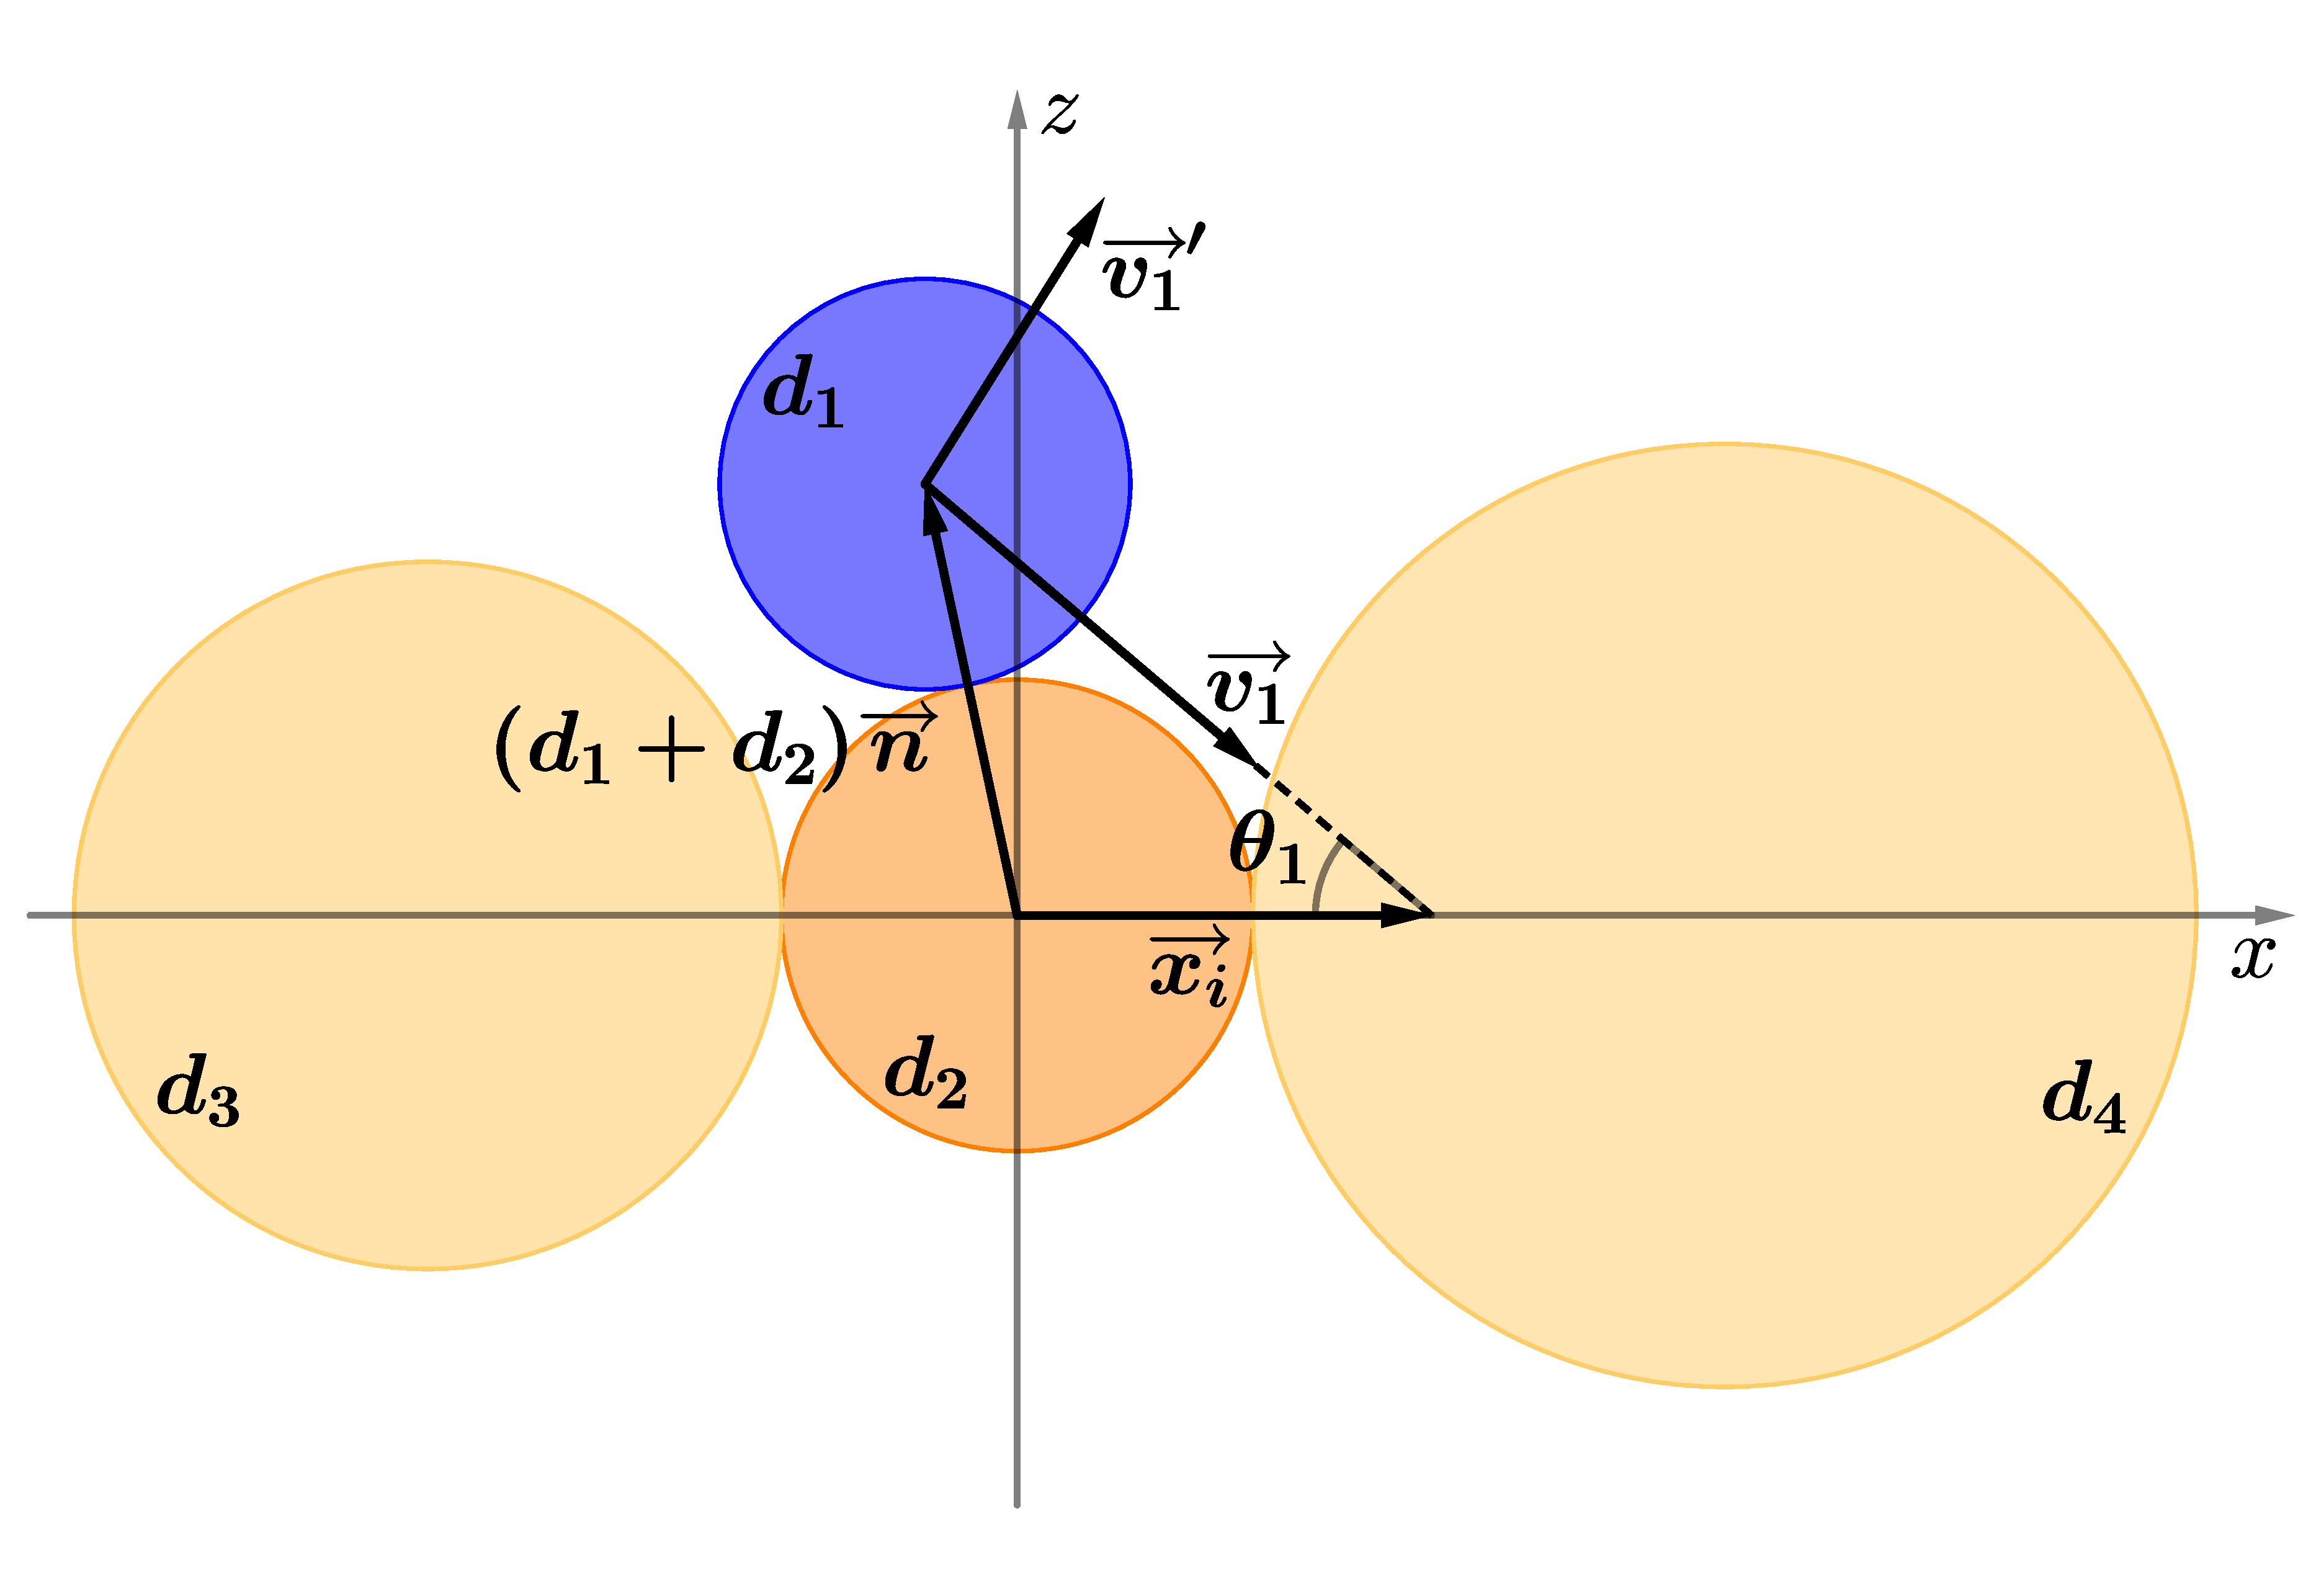
\includegraphics[width=0.8\textwidth]{fig1.pdf}
    \caption{Illustration of the collision between a particle and the bed.}
    \label{fig1}
\end{figure}

As shown in \ref{fig1}, a impactor with diameter $d_1$ collides with a bed particle with diameter $d_2$. The impact velocity of the impactor is $\overrightarrow{v_1}$, and the rebound velocity is $\overrightarrow{v_1}'$. The angle between the impact velocity and the horizontal plane is $\theta_1$. After locating the center of the bed particle $d_2$ at the origin of the coordinate system, a vector $\overrightarrow{x_i}$ from the origin to the location $(x_i, 0)$ is defined to denote the impact location. With this impact location, the components of the rebound velocity $\overrightarrow{v_1}'$ can be expressed as (L\"ammel et al., 2017)
\begin{equation}
    \frac{v_{1x}'}{\overrightarrow{v_1}} = - \alpha \cos\theta_1 + (\alpha + \beta) x_i^2 \sin^2\theta_1\cos\theta_1 + (\alpha + \beta) x_i \sin^2\theta_1 \sqrt{1 - x_i^2\sin^2\theta_1}, \label{eq:v1x}
\end{equation}
\begin{equation}
    \frac{v_{1z}'}{\overrightarrow{v_1}} = \alpha \sin\theta_1 - (\alpha + \beta) x_i^2 \sin^3\theta_1 + (\alpha + \beta) x_i \sin\theta_1\cos\theta_1 \sqrt{1 - x_i^2\sin^2\theta_1}. \label{eq:v1z}
\end{equation}
Obviously, for a specific impact velocity $\overrightarrow{v_1}$, the function $F(\overrightarrow{v_1}')$ of the particle rebound velocity is determined by $x_i$. Forthermore, the average of $F$ over all possible impact locations can be expressed as
\begin{equation}
    \overline{F} = \frac{1}{x_{i, max} - x_{i, min}} \int_{x_{i,min}}^{x_{i,max}} F \diff x_i,
\end{equation}
where the integration limits are determined by the diameters of the impactor and the bed particles. The leftmost limit corresponds to two pausible cases: a) the impactor moves tangentially through the left neighbor of the centering particle; b) the impactor impact the centering particle and the left neighbor at the same time. Then the leftmost limit $x_{i,min}$ can be expressed as
\begin{equation}
    x_{i, min} = \begin{cases}
        d_{13}\csc\theta_1 - d_{12}, & \theta \leq \theta_c \\
        \frac{d_2}{2}, & \text{if } d_1 > d_2
    \end{cases}
\end{equation}

% 示例:多行公式对齐
%\begin{align}
%    \frac{\pdiff f}{\pdiff t} &= \frac{\pdiff}{\pdiff t}\int_a^b g(x,t)\diff x \\
%    &= \int_a^b \frac{\pdiff g}{\pdiff t}\diff x
%\end{align}
%
%% 示例:分段函数
%\[
%    f(x) = \begin{cases}
%        x^2, & x \geq 0 \\
%        -x^2, & x < 0
%    \end{cases}
%\]
%
%% 示例:矩阵
%\[
%    \begin{bmatrix}
%        a_{11} & a_{12} \\
%        a_{21} & a_{22}
%    \end{bmatrix}
%    \begin{bmatrix}
%        x_1 \\
%        x_2
%    \end{bmatrix} =
%    \begin{bmatrix}
%        b_1 \\
%        b_2
%    \end{bmatrix}
%\]
%
%\section{推导过程}
%% 这里可以继续您的推导...

\end{document} 